\prob{
    Find each of the following:
    \begin{enumerate}[label=(\roman*)]
        \item all self-dual uniform matroids;
        \item all identically self-duall uniform matroids;
        \item all self-dual graphic matroids on six or fewer elements;
        \item all identically self-dual graphic matroids on six or fewer elements;
        \item an infinite family of simple graphic self-dual matroids.
    \end{enumerate}
}
\begin{proof}$\,$\pn
    \begin{enumerate}[label=(\roman*)]
        \item 
            Let $U_{n,m}$ be an uniform matroid.\pn
            
            Lets asume that it is self-dual. As
            any basis $B$ for $U_{n,m}$ has size $n$, if it is going to be self-dual,
            then its complement must have size $n$ as well. This means that $m = 2n$.\pn
            
            Now lets suppose that $m = 2n$. So, any subset of size $n$ is a basis for $U_{n,m}$,
            but it is also true that any subset of size $n$ is the complement of another subset
            of size $n$ and then, any basis is the complement of another basis. Then $U_{n,m}$ is
            not only self-dual, but also identically self-dual.
        \item 
            Just as we saw above, if an uniform matroid is self-dual, then it is identically self-dual, and
            an uniform matroid $U_{n,m}$ is self-dual if and only if $m = 2n$.
            
        \item 
            It is clear that if a matroid is to be self-dual, then its size must be two times
            the size of any of its basis (any forest that is not contained in any other forest). 
            This means that there are only self-dual graphic matroids with an even number of edges. \pn
            
            Lemma 2.3.7 from~\cite{Oxley} stays that if $G^*$ is a geometric dual of the planar graph $G$, then
            $M(G^*) \cong M^*(G)$. In particular for self-dual matroids we will have that $M(G^*) \cong M^*(G) \cong M(G)$.
            
            From now on we will use this fact to look for the remaining self-dual matroids. As the maximum size of these matroids
            is $6$ and $K_4$ is a complete planar graph with 6 edges, then every one of the matroids will have a planar representation. 
            And the previously mentioned lemma will let us work with graph representations instead of a complicated structure of 
            subsets and its intersections.\pn
            
            Also, notice that if $G$ is a planar graph. And $H = G \cup G^*$, then $M(H)$ is self-dual. The only
            trick is to send $M(G)$ to $M(G)$ in the dual and $M(G^*)$ to $M(G^*)$ in the dual.\pn
            
            Considering this. We will try to find self-duality through blocks (2-connected maximal subgraphs) when it is possible.
            Also, the drawings will be done thinking of these, we are going to separate in as many blocks as possible, given that
            it will not affect the resultant matroid.\pn
            
            We will try to order our analysis by the size of the maximum cycle contained in a graph or its dual matroid. And for this
            remember that the dual of a $n$-cycle is a set of $n$ edges all of them parallel to each other.\pn            
            
            \textbf{2 edges}:\pn
                \begin{itemize}
                    \item \textbf{No cycles.}
                        There is no such graph. If a graph has no cycles, then its dual contains only loops (which are cycles).
                        This will happen in any of the other graphs so we are not going to list this case anymore.
                    
                    \item \textbf{Cycles of size at most 1.}
                        If there has to be a loop, then it has to be an edge that is not a loop. The loop will be maped to the dual of
                        the edge that is not a loop and viceversa. This one is not identically self-dual. 
                        
                        \begin{figure}[H]
                            \begin{center}
                            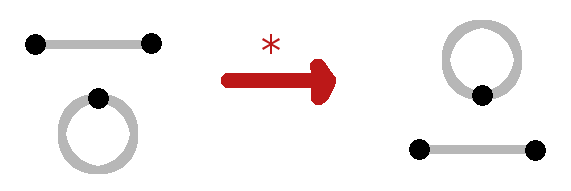
\includegraphics[width=5cm]{Test2/Problem1/1_0.png}
                            \end{center}
                            \caption{self-dual graphic matroid representation}
                            \label{t2:p1_1_0.png}  
                        \end{figure}\pn
                        
                    \item \textbf{Cycles of size at most 2.}
                        There is only one way to get a cycle of size two with two edges, and it is easy to see that it has not only
                        a self-dual matroid but an identically auto-dual matroid.
                        
                        \begin{figure}[H]
                            \begin{center}
                            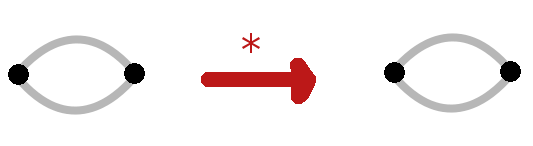
\includegraphics[width=5cm]{Test2/Problem1/2.png}
                            \caption{identically self-dual graphic matroid representation}
                            \label{t2:p1_2.png}
                            \end{center}                        
                        \end{figure}\pn
                \end{itemize}
                  
                There cannot be larger cycles with only 3 edges.\pn
            \textbf{4 edges}:\pn
            
                \begin{itemize}
                   \item \textbf{Cycles of size at most 1.}
                        Again. For every loop ther must be an edge that is not a loop. And for every edge that is not a loop there 
                        must be a loop. So the only posibility left is to have two loops and two edges that are not loops.
                        
                        \begin{figure}[H]
                            \begin{center}
                            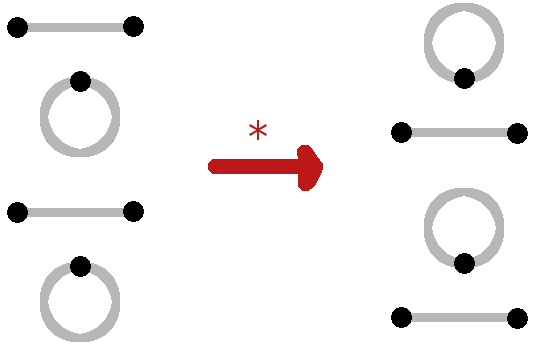
\includegraphics[width=5cm]{Test2/Problem1/1_0-1_0.png}
                            \end{center}                        
                        \end{figure}\pn
                        
                   \item \textbf{Cycles of size at most 2.}
                        If we have a block as in \ref{t2:p1_2.png}, then, under the matroid isomorphisim are two posibilities,
                        that such block is mapped into itself, or that it is mapped into another block.
                        
                        If it is mapped into another block, then the other block must be essentialy the same graph and then
                        whe have something like
                        \begin{figure}[H]
                            \begin{center}
                            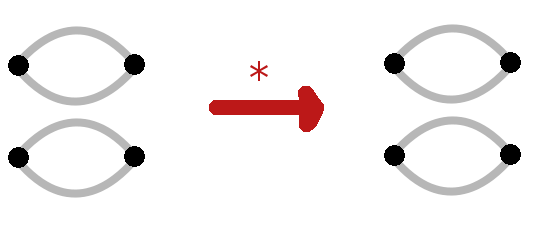
\includegraphics[width=5cm]{Test2/Problem1/2-2.png}
                            \end{center}                            
                            \caption{identically self-dual graphic matroid representation}
                            \label{t2:p1_2-2.png}                        
                        \end{figure}\pn
                        
                        (Notice that this will result in an identically self-dual matroid also. Every forest is a pair of
                        non-parallel edges, and its complement is also a pair of non-parallel edges.)\pn
                        
                        If the first block is mapped into itself, then the other block must be mapped into itself also.
                        Then the other block must be a representation of a self-dual matroid on 2 edges. And then, there are
                        two posibilities. If the other block is like in \ref{t2:p1_2.png}, then we will obtain again 
                        \ref{t2:p1_2-2.png}. If the other block is like \ref{t2:p1_1_0.png} then we will obtain something like
                        \begin{figure}[H]
                            \begin{center}
                            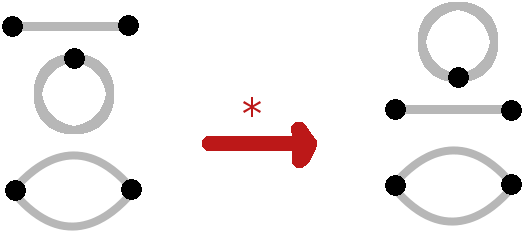
\includegraphics[width=5cm]{Test2/Problem1/2-1_0.png}
                            \end{center}                            
                            \caption{self-dual graphic matroid representation}
                            \label{t2:p1_2-1_0.png}                        
                        \end{figure}\pn
                        
                        (Notice that this could not be identically self-dual. As it has loops, any loop will be in a cobasis, but no
                        basis contains loops.)\pn
                        
                    \item \textbf{Cycles of size at most 3.}
                        A graph that will represent a self-dual matroid and that has a 3-cycle and at most 4 edges, must have at most
                        one block. Otherwise, on block must be the triangle, but a triangle is not self-dual and could not be mapped 
                        in the other block that only could have 1 edge.\pn
                        
                        This gives us essentially only one opportunity. A triangle adding a parallel edge to one of its edges.
                        An isomorphism would be sending the simple edges to the parallel edges and the parallel edges to the simple 
                        edges. The two simple edges form a set that intersects any of the basis of the matroid, so it is a cocircuit. 
                        The proposed isomorphism send that cocircuit to a circuit in the original matroid. The two parallel edges along 
                        with any of the simple edges form another set that intersects any of the basis of the original matroid, so it 
                        is another cocircuit in the dual matroid. Those edges are sent to a triangle in the original matroid. There 
                        are two of these cocircuits and each one is sent two one of the two possible triangles in the original matroid.
                        Any basis formed for a simple edge and one of the two parallel edges has as complement the other simple edge 
                        and the other parallel edge, and under the proposed isomorphism any of such basis are sent to other of the 
                        same type. The only other basis that is left is the one that consits of the two simple edges, and they are 
                        sent to the pair of parallel edges, which is independent in the dual matroid. We have proved so far that this 
                        isomorphism sends any of the basis in the original matroid to a basis in the dual matroid and any cocircuit 
                        to a circuit in the original matroid. Then such isomorphism is a matroid isomorphism between the graphic matroid 
                        and its dual.\pn
                        
                        \begin{figure}[H]
                            \begin{center}
                            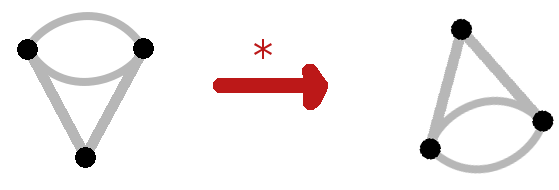
\includegraphics[width=5cm]{Test2/Problem1/4.png}
                            \end{center}                            
                            \caption{self-dual graphic matroid representation}
                            \label{t2:p1_4.png}                        
                        \end{figure}\pn
                        
                        This could not be identically self-dual as it has a cobasis that contains parallel edges.
                        
                    \item \textbf{Cycles of size at most 4.}
                        There is none, as the only cycle of size 4 has 4 edges, and as the 4-cycle is not self-dual, there cannot be
                        self-dual matroids with 4-elements and 4-cycles.
                \end{itemize}
    
                There cannot be larger cycles with only 4 edges.\pn
            \textbf{6 edges}:\pn
            MISSING!
        \item 
            Any graph on six or fewer elements obtained from a forest adding a parallel edge to each edge in the forest.
            We have proved this in the last part, indicating which of the self-dual matroids are identically self-dual or non-identically self-dual.
            
        \item 
            Any wheel. Proof in [\ref{p11}]
    \end{enumerate}
\end{proof}